% Local and remote flow routes; one shared public source.
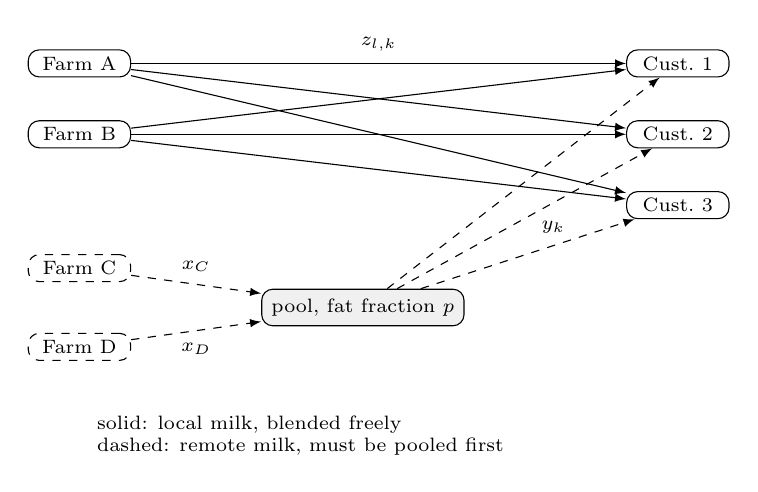
\begin{tikzpicture}[scale=1.0,>=latex,
    every node/.style={font=\scriptsize},
    farm/.style={draw,rounded corners,inner sep=2.5pt,minimum width=13mm}]
  % local farms, upper left; remote farms, lower left
  \node[farm]        (A) at (0,3.6) {Farm A};
  \node[farm]        (B) at (0,2.7) {Farm B};
  \node[farm,dashed] (C) at (0,1.0) {Farm C};
  \node[farm,dashed] (D) at (0,0.0) {Farm D};
  % the pool, well clear of the local -> customer arrows above it
  \node[draw,rounded corners,fill=black!6,inner sep=3.5pt] (P) at (3.6,0.5)
       {pool, fat fraction $p$};
  % customers, right, all above the pool
  \node[farm] (K1) at (7.6,3.6) {Cust.\ 1};
  \node[farm] (K2) at (7.6,2.7) {Cust.\ 2};
  \node[farm] (K3) at (7.6,1.8) {Cust.\ 3};
  % remote -> pool. Labels ABOVE and BELOW the line, at the midpoint, on a
  % 2.3cm run -- short runs put the label inside the node box, which is what
  % the first draft of this figure did.
  \draw[->,dashed] (C) -- node[above=1pt,midway] {$x_{\text{C}}$} (P);
  \draw[->,dashed] (D) -- node[below=1pt,midway] {$x_{\text{D}}$} (P);
  % pool -> customers
  \draw[->,dashed] (P) -- node[above=1pt,pos=0.62] {$y_k$} (K3);
  \draw[->,dashed] (P) -- (K2);
  \draw[->,dashed] (P) -- (K1);
  % local -> customers
  \draw[->] (A) -- node[above=1pt,pos=0.5] {$z_{l,k}$} (K1);
  \draw[->] (A) -- (K2);
  \draw[->] (A) -- (K3);
  \draw[->] (B) -- (K1);
  \draw[->] (B) -- (K2);
  \draw[->] (B) -- (K3);
  \node[anchor=north west,align=left] at (0.1,-0.75)
       {solid: local milk, blended freely\\
        dashed: remote milk, must be pooled first};
\end{tikzpicture}
